
% \section{\DSU}
% \ShowTOC[currentsection]

\begin{frame}{\DSU{} - System overview}%{A Sub-title is optional}
\begin{center}%
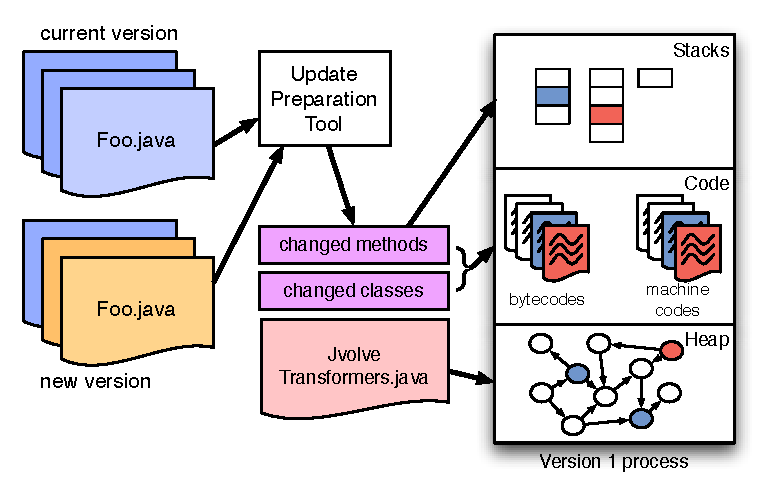
\includegraphics[width=0.93\paperwidth]{images/developers-view}%
\end{center}%
\end{frame}

% \begin{frame}{Update Model}%{A Sub-title is optional}
% \begin{itemize}
% \item Update happens in one fell swoop
% \item Simple to reason about
% \item Code
%   \begin{itemize}
%   \item Old code before the update
%   \item New code after the update
%   \end{itemize}
% \item Data
%   \begin{itemize}
%   \item \emph{Representation consistency} (all values of a type \\
%         correspond to the latest version)
%   \item Support a transformation function to convert objects to conform to
%         their new definition
%   \end{itemize}
% \end{itemize}
% \end{frame}

\newcommand{\removed}[1]{\textcolor{red}{- #1}}
\newcommand{\addedxx}[1]{\textcolor{OliveGreen}{+ #1}}

\begin{frame}[fragile]{Supported updates}%{A Sub-title is optional}
\begin{itemize}
\item Changes within the body of a method \\
\begin{footnotesize}
\begin{semiverbatim}
  public static void main(String args[]) \{
    System.out.println("Hello, World.");
\addedxx{  System.out.println("Hello again, World.");}
  \}
\end{semiverbatim}
\end{footnotesize}
\item Class signature updates
  \begin{itemize}
  \item Add, remove, change the type signature of fields and methods
  \end{itemize}
\begin{footnotesize}
\begin{semiverbatim}
  public class Line \{
\removed{  private final Point2D p1;}
\addedxx{  private final Point3D p1;}
    ...
  \}
\end{semiverbatim}
\end{footnotesize}
% \item Changes can occur at any level of the class hierarchy
\item Signature updates require an object transformer function
\end{itemize}
\end{frame}


% \begin{frame}{Division of Labor}%{A Sub-title is optional}
% I think this slide should get killed. Let me know what you think.
% \begin{itemize}
% \item Developer
%   \begin{itemize}
%   \item Write the old and new versions
%   \item Write class/object transformation functions for classes that
%         changed (optional)
%   \item Testing (both the application and the update)
%   \end{itemize}
% \item \DSU{} system
%   \begin{itemize}
%   \item Update Preparation Tool (UPT) identifies differences between versions
%     \begin{itemize}
%     \item Identifies classes that have changed signature (added or removed
%           field/method)
%     \item Identifies method body changes
%     \end{itemize}
%   \item \DSU{} VM handles the update
%   \end{itemize}
% \end{itemize}
% \end{frame}

% \ShowTOC
% \subsection{Developer's role}

% \newcommand{\ExampleCodeSize}{footnotesize}

% \newcommand{\removed}[1]{\textcolor{red}{- #1}}
% \newcommand{\addedxx}[1]{\textcolor{OliveGreen}{+ #1}}

\begin{frame}[fragile,shrink=5]{Example of an update (JavaEmailServer)}%{A Sub-title is optional}
\begin{\ExampleCodeSize}
\begin{semiverbatim}
  public class User \{
    private final String username, domain, password;
\removed{  private String[] forwardAddresses;}
\addedxx{  private EmailAddress[] forwardAddresses;}
    public User(...) \{...\}
    public String[] getForwardedAddresses() \{...\}

    public void setForwardedAddresses(String[] f) \{...\}

  \}

  public class ConfigurationManager \{
    private User loadUser(...) \{
       ...
       User user = new User(...);
       String[] f = ...;

       user.setForwardedAddresses(f);
       return user;
    \}
  \}
\end{semiverbatim}
\end{\ExampleCodeSize}
\end{frame}


% \begin{frame}[fragile,shrink=5]{Example of an update (JavaEmailServer)}%{A Sub-title is optional}
% \begin{\ExampleCodeSize}
% \begin{semiverbatim}
% public class User \{
%   private String username, domain, password;
%   private \sout{String[]} EmailAddress[] forwardAddresses;
%   public \sout{String[]} EmailAddress[] getForwardedAddresses() \{...\}
%   public void setForwardedAddresses(\sout{String[]} EmailAddress[] f) \{...\}
% \}
% 
% public class ConfigurationManager \{
%   private User loadUser(...) \{
%      ...
%      User user = new User(...);
%      \sout{String[]} EmailAddress[] f = ...;
%      user.setForwardedAddresses(f);
%      return user;
%   \}
% \}
% 
% \end{semiverbatim}
% \end{\ExampleCodeSize}
% \end{frame}

\begin{frame}[fragile,shrink=5]{Example of an update (JavaEmailServer)}%{A Sub-title is optional}
\begin{\ExampleCodeSize}
\begin{semiverbatim}
  public class User \{
    private final String username, domain, password;
\removed{  private String[] forwardAddresses;}
\addedxx{  private EmailAddress[] forwardAddresses;}
    public User(...) \{...\}
\removed{  public String[] getForwardedAddresses() \{...\}}
\addedxx{  public EmailAddress[] getForwardedAddresses() \{...\}}
\removed{  public void setForwardedAddresses(String[] f) \{...\}}
\addedxx{  public void setForwardedAddresses(EmailAddress[] f) \{...\}}
  \}

  public class ConfigurationManager \{
    private User loadUser(...) \{
       ...
       User user = new User(...);
\removed{     String[] f = ...;}
\addedxx{     EmailAddress[] f = ...;}
       user.setForwardedAddresses(f);
       return user;
    \}
  \}
\end{semiverbatim}
\end{\ExampleCodeSize}
\end{frame}

\begin{frame}[fragile,shrink=5]{Example of an update (JavaEmailServer)}%{A Sub-title is optional}
\mode<beamer> {
\begin{textblock*}{46mm}[0,0](79mm,20mm)
\begin{block}{}
Stub generated by UPT for the old version
\end{block}
\end{textblock*}
\only<1>{
\begin{textblock*}{46mm}[0,0](79mm,48mm)
\begin{block}{}
Default transformer copies old fields, initializes new ones to
\texttt{null}
\end{block}
\end{textblock*}}
}
\begin{small}
\begin{semiverbatim}
public class v131_User \{
  private final String username, domain, password;
  private String[] forwardAddresses;
\}
public class JvolveTransformers \{
 ...
 public static void jvolveClass(User unused) \{\}
 public static void jvolveObject(User to, v131_User from) \{
    to.username = from.username;
    to.domain = from.domain;
    to.password = from.password;
    // to.forwardAddresses = null;
    \uncover<2>{int len = from.forwardAddresses.length;
    to.forwardAddresses = new EmailAddress[len];
    for (int i = 0; i < len; i++) \{
      to.forwardAddresses[i] =
        new EmailAddress(from.forwardAddresses[i]);
}\}\}\}

\end{semiverbatim}
\end{small}
\end{frame}


% \begin{frame}[fragile,shrink=5]{Example of an update (JavaEmailServer)}%{A Sub-title is optional}
% \begin{\ExampleCodeSize}
% \begin{semiverbatim}
% public class User \{
%   private String username, domain, password;
%   private \sout{String[]} EmailAddress[] forwardAddresses;
%   public \sout{String[]} EmailAddress[] getForwardedAddresses() \{...\}
%   public void setForwardedAddresses(\sout{String[]} EmailAddress[] f) \{...\}
% \}
% 
% public class ConfigurationManager \{
%   private User loadUser(...) \{
%      ...
%      User user = new User(...);
%      \sout{String[]} EmailAddress[] f = ...;
%      user.setForwardedAddresses(f);
%      return user;
%   \}
% \}
% 
% \end{semiverbatim}
% \end{\ExampleCodeSize}
% \end{frame}

% \begin{frame}{Object Transformers}%{A Sub-title is optional}
% \begin{itemize}
% \item ``Transform'' objects to correspond to the new version
% \item Functions generated by the Update Preparation Tool (UPT)
% \item Accept old object and new objects as parameters
% \item Default transformer copies old fields and initializes new ones to
% \texttt{null}
% \item User can optionally modify these functions
% \end{itemize}
% \end{frame}
